%\fontfamily{ptm}\selectfont
\documentclass[11pt]{article}
\usepackage{hyperref}
\hypersetup{
  colorlinks=true,
  linkcolor=blue,
  urlcolor=blue
}
\renewcommand{\sfdefault}{ptm}
\title{Ada on the ST SensorTile}
\author{
  %\large
  \textsc{Hedley Rainnie}
  \mbox{}\\ %
  \url{http://hrrzi.com}\\
  Cupertino, CA 95014\\
  \mbox{}\\ %
}
%\documentclass{acmconf}

\usepackage[paper=a4paper,dvips,top=1.5cm,left=1.5cm,right=1.5cm,
    foot=1cm,bottom=1.5cm]{geometry}

\usepackage{times}
\usepackage{graphicx}
\usepackage[fleqn]{amsmath}
\usepackage{amsfonts}
\usepackage{amssymb}
\usepackage{amsthm}
\usepackage{amsopn}
\usepackage{xspace}
\usepackage{xcolor}
\usepackage{placeins}
\usepackage{array}
\usepackage{epsfig}
\usepackage{float}
\usepackage{siunitx}
\usepackage{tikz}
\def\checkmark{\tikz\fill[scale=0.4](0,.35) -- (.25,0) -- (1,.7) --
  (.25,.15) -- cycle;}
\usepackage{enumitem}
\usepackage{dirtree}
\usepackage[T1]{fontenc}
\DeclareSIUnit[number-unit-product = {}]{\inchQ}{\textquotedbl}
\DeclareSIUnit[number-unit-product = {\thinspace}]{\inch}{in}
%\usepackage{url}
%\usepackage{algpseudocode}

\numberwithin{figure}{section}

\usepackage{labels} %
\usepackage{equation}
%\usepackage{prog2tex}

\usepackage{listings}
\usepackage{color}
%\usepackage{courier}
%\usepackage{droidsans}
\usepackage{bera}
\definecolor{darkorange}{rgb}{1.0,0.55,0.0}
\definecolor{orange}{rgb}{1.0,0.64,0.0}
\definecolor{cyan}{rgb}{0.0,1.0,1.0}
\definecolor{blue}{rgb}{0.0,0.0,1.0}
\lstset{
   breaklines=yes,
   language=Ada,
   commentstyle=\color{orange},
   keywordstyle=\color{blue},
   basicstyle=\ttfamily
}
\newenvironment{excerpt}{\begin{quote}\begin{minipage}\textwidth}{\end{minipage}\end{quote}}

\setcounter{topnumber}{0}
\setcounter{bottomnumber}{0}
\setcounter{totalnumber}{20}
\renewcommand{\textfraction}{0.01}

\begin{document}

\maketitle

\begin{abstract}
This project is a submission for the Make with Ada contest. Ada is
shown in three activities, one as a server connected to ST's BLE app,
then as a server to a Raspberry Pi3 and finally as client and server
SensorTiles. All communication is done using ST's BLE chip via Ada
coded drivers. Numerous sensors are present and almost all are
used/initialized. For the client/server demo, a musical instrument,
\textit{AdaTheremin} is created. This is in the spirit of L\'eon
Theremin's eponymous creation but in no way is it to be a betterment.
It is realized by using a fixed magnet and its proximity to and motion
of the SensorTile server. This proximity and motion is beamed to the
client node where audio may be heard that is derived from the incoming
data. This project paves the way for Ada+BLE on ST's new STM32WB SoC
(CM4F + CM0(BLE)) coming in March.
\end{abstract}

\section{Introduction}
To describe the effort for this project I visualize a cartoon where a
hapless fool has a teaspoon to move a mound of sand, as the frame pans
back, the mound turns out to be larger and then impossibly
larger. This is the feeling you may experience if you are to try a
port of Ada to a SensorTile using just weekends and holidays to do
it. Here is a cartoon from my sister Felicity that captures this:

\begin{figure}[H]
\centering
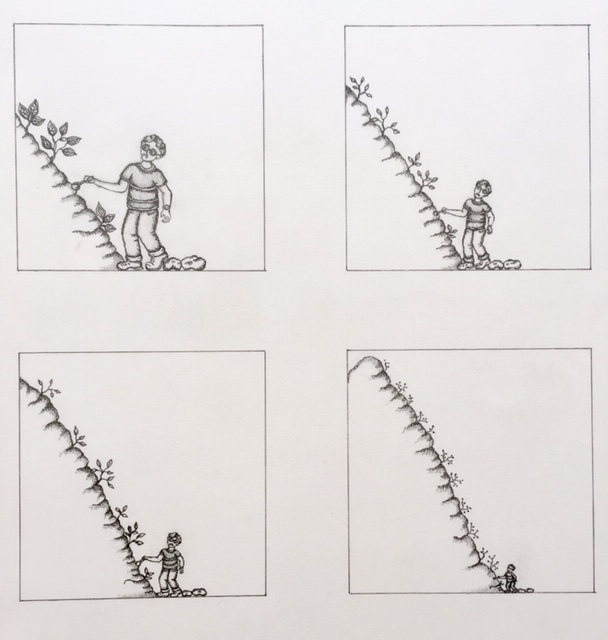
\includegraphics[scale=0.6]{Flip_Cartoon.jpg}
\caption{by Felicity Rainnie depicting the impossible task}
\label{Figure:Flip_Cartoon.jpg}
\end{figure}

Like all such tasks though, just stay focused and keep working
away little by little at the problem. Slowly but surely items that
seem intractable become tractable and progress gets made. I bought a
SensorTile a year ago and then added another. They are not cheap, 80\$
each. Out of the package you can run a SensorTile on one of two
cradles, a small one which fits in a plastic holder and can be a
wearable as it is powered by either external connections or the cradle
\SI{105}{\milli\ampere\hour} battery. The other cradle is has Arduino
headers and sports a USB connector plus a 3.5mm audio jack. The
smaller cradle has two off SensorTile sensors shown in the table below
as S1 \& S2, the larger cradle, just one I2C peripheral, the PCM1774
audio codec (from TI no less, I guess ST doesn't have that one).
\clearpage
\begin{figure}[!htbp] % client & slave
\centering
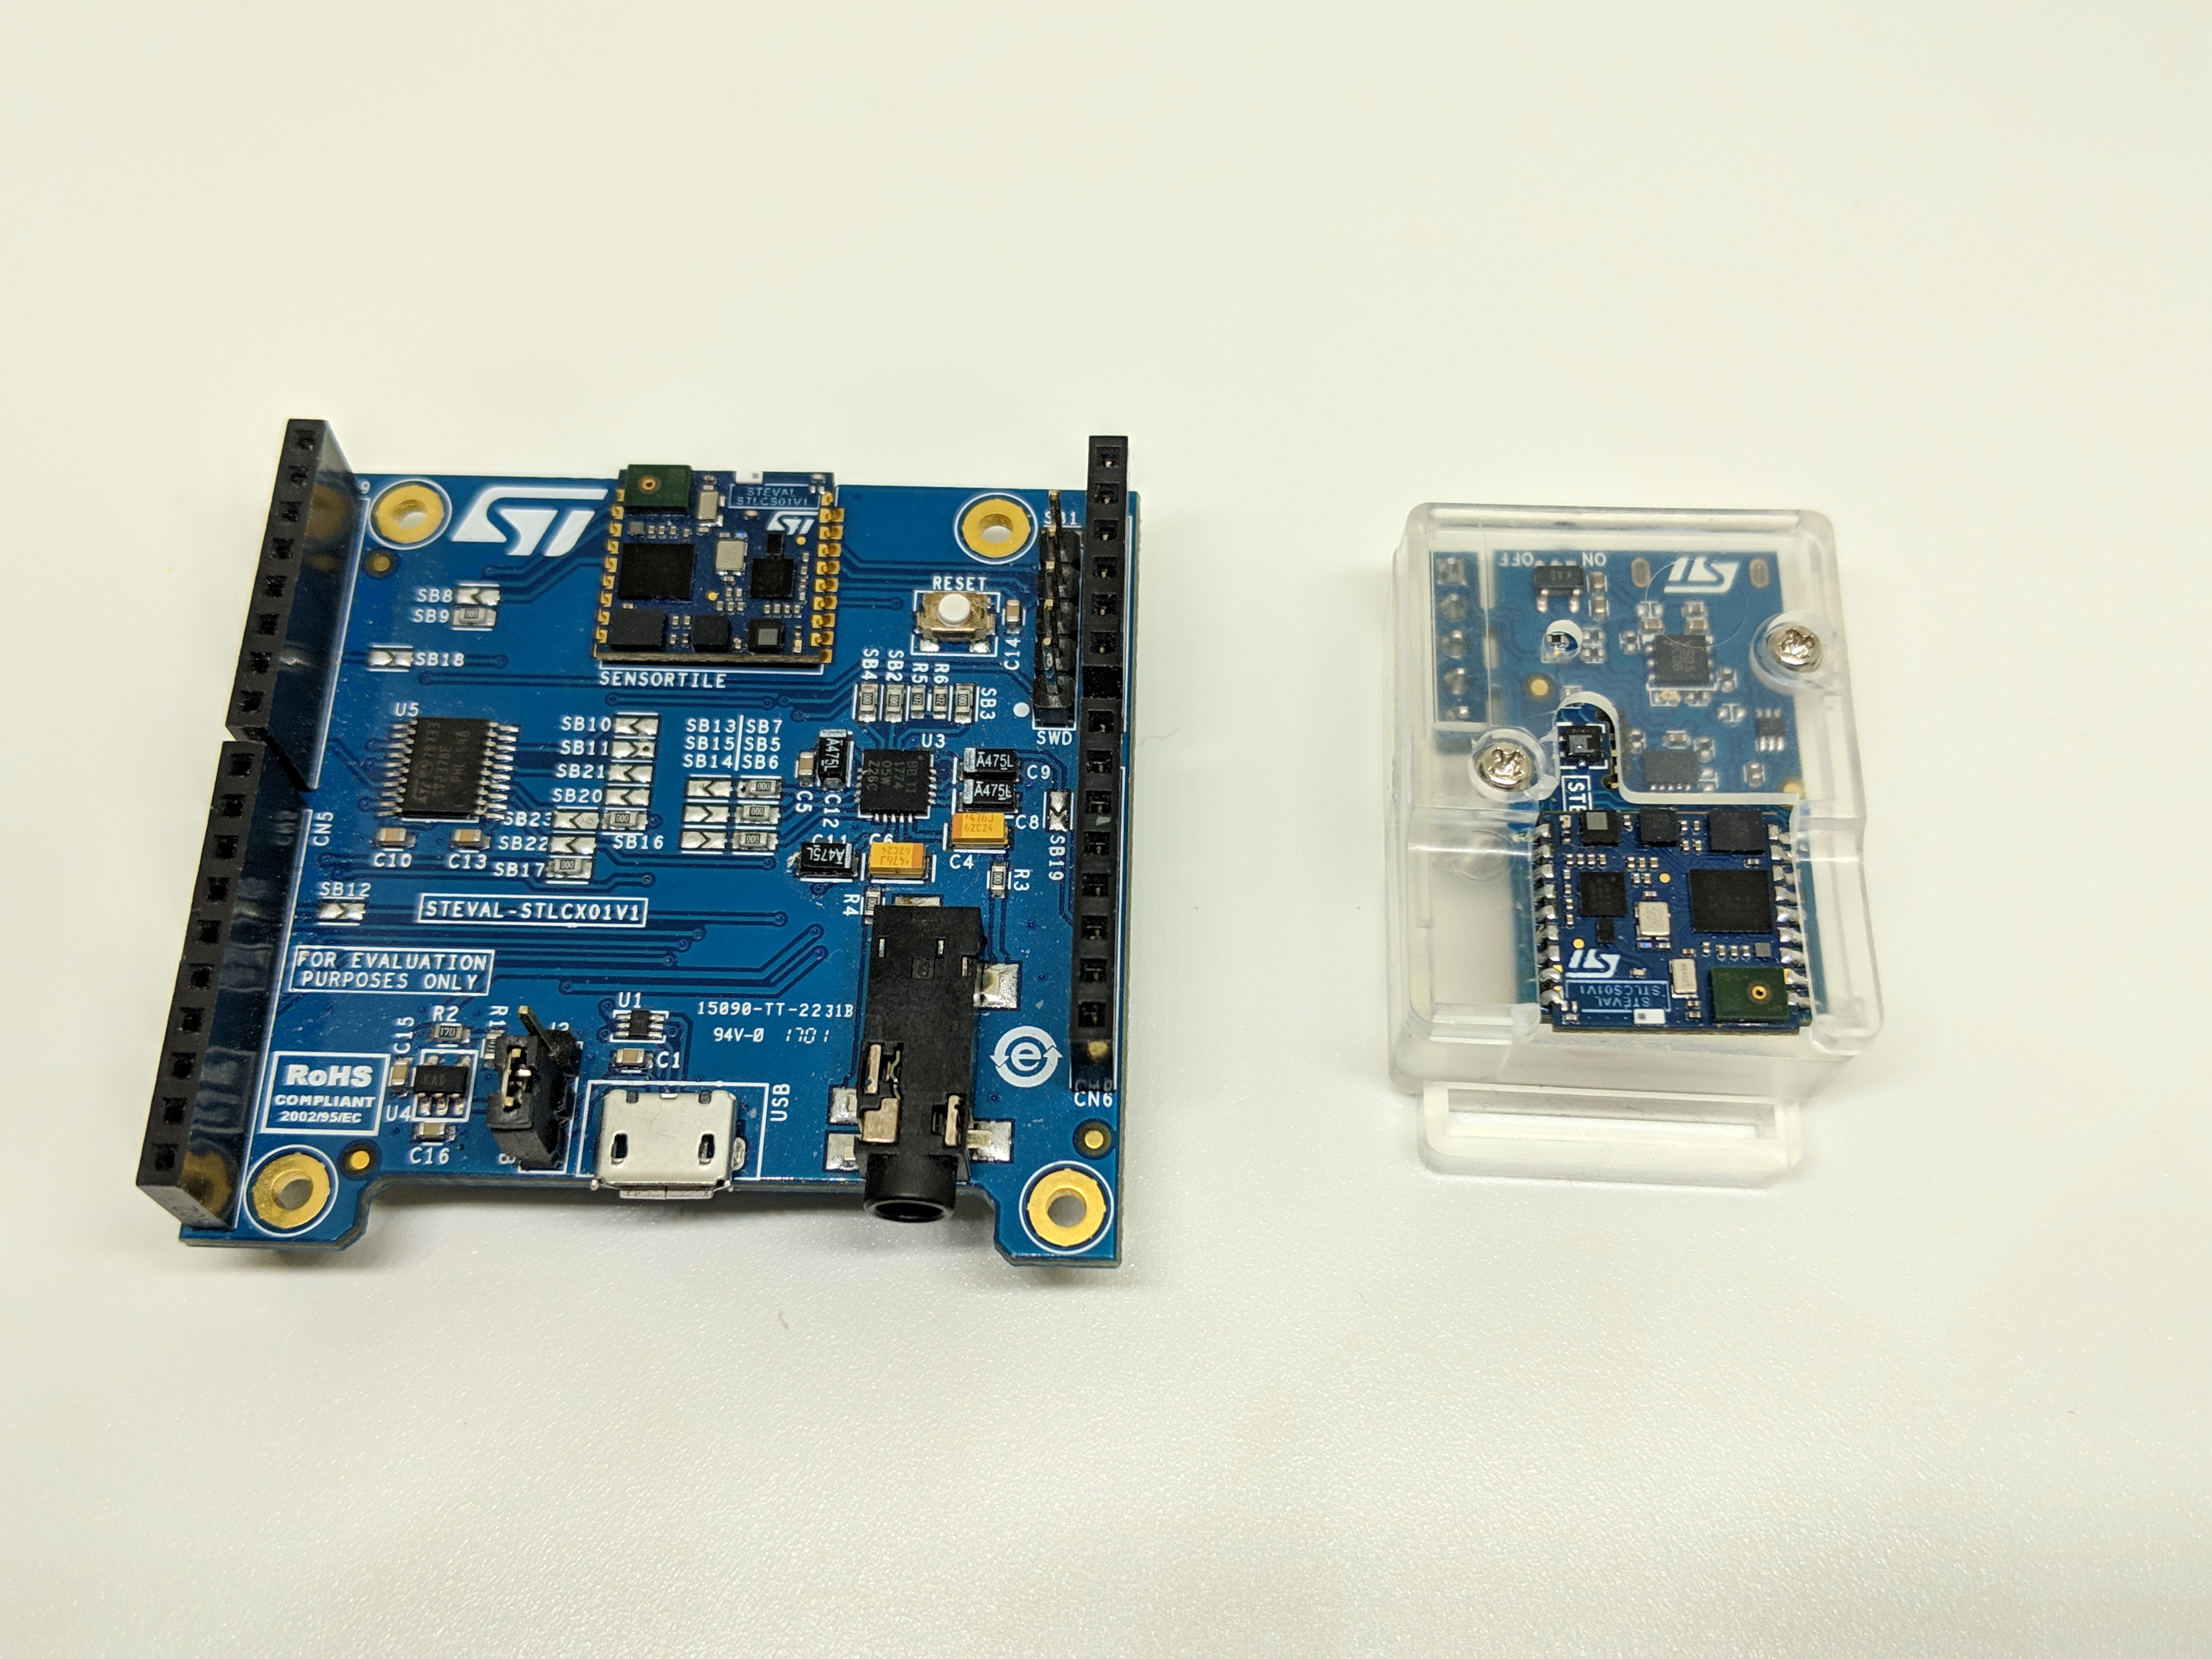
\includegraphics[scale=0.1]{ST2.jpg}
\caption{SensorTiles and cradles shown as Client on left, Server on right}
\label{Figure:ST2.jpg}
\end{figure}

\clearpage
\begin{figure}[!htb] % SensorTile
\centering
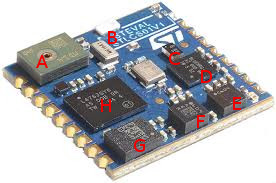
\includegraphics[scale=1.0]{sensortile2.jpg}
\caption{The ST SensorTile. 13.5mm square}
\label{Figure:SensorTile}
\end{figure}

\begin{table}[h]
\begin{tabular}{|l|l|l|l|}
\hline
Reference   & Device   & Description & Interface\\ \hline
A & MP34DT04 & MEMS audio sensor digital microphone & DFSDM \\ \hline
B & ANT1 & BT Antenna & -\\ \hline
C & BALF & \SI{50}\ohm \ BT Balun & - \\ \hline
D & BlueNRG-MS & BLE network processor & SPI1 4 wire \\ \hline
E & LPS22HB & MEMS pressure sensor & SPI2 3 wire\\ \hline
F & LSM303AGR & eCompass, 3D accelerometer \& 3D magnetometer & SPI2
3 wire \\ \hline
G & LSM6DSM & 3D accelerometer \& 3D gyroscope & SPI2
3 wire \\ \hline
H & STM32L476 & ARM Cortex-M4F 32-bit microcontroller & -  \\ \hline
Server/Client   & Device   & Description & Interface\\ \hline
S1 & STC3115 & Battery monitor & I2C3\\ \hline
S2 & HTS221 & Humidity sensor & I2C3\\ \hline
C1 & PCM1774 & Audio codec & I2C3\\ \hline
\end{tabular}

\end{table}
\FloatBarrier
%{
%\fontfamily{bera}\selectfont
%\lstinputlisting{aqi3.adb}
%}
%Lets see if it switches back to serif fonts for this sentence.
\section{First steps}
The first item of business was to assess the target. For the past Make
with Ada project, I had ported the Ada\_Drivers\_Library to the
STM32L432 this is a relatively small SoC and has a reduced amount of
almost everything. Same CPU though, the CM4F. This SensorTile SoC
however had lots of peripherals but they were all connected quite
specifically to perform the SensorTile function. So the SensorTile
schematics were invaluable. From the schematic, its easy to see what
pins are used for sensor interfacing. ST also provides SVD files for
each STM32 SoC they produce. This file is
\textcolor[rgb]{1.0,0.84,0.0}{\textbf{gold}} and without it, I doubt this
project could have been done (at least using the methodology I like to use).

One word of caution here, a SensorTile is only 13.5mm square, it
is 100\% composed of high density BGA parts. There are
\textcolor[rgb]{1.0,0.0,0.0}{\textbf{no}} exposed traces between the packages. This means that no-one is going
to be connecting up a Saleae analyzer to probe traffic to and from the
SoC to the sensors. The upshot is, everything useful in the bringup of
this target in Ada must be obtained over the SWD port. Which makes SWD
debug and tools associated with that absolutely critical to project
success.
\subsection{SWD}
The SensorTile uses SWD for its debug communication. Out of the box,
there is no way to immediately connect to it unless you have a donor
STM32 series with its STLinkV2.1 (don't we all?). So, pop off two
jumpers on a STM32F401 Nucleo board and the SWD connector is no longer
connected to the STM32F4 part but to whatever you have on the end of
the connector. Helpfully, in the SensorTile blister pack is a 5 pin
cable for just this bridge. Once this is connected up, OpenOCD (with
some small mods to understand the parts flash layout) can now be
connected to the target. Here we see the cfg file. The first two lines
allow selection of STLinkV2.1 or STLinkV2 the former is for the board
to board bridge, the latter for use with an inexpensive STLink that
can be had on eBay for about \$2.50. I like the inexpensive one as its
small and can be transported easily, see it pictured below after the
cfg file.

{
\fontfamily{bera}\selectfont
\lstinputlisting{sensortile.cfg}
}

\begin{figure}[!htbp] % sensortile
\centering
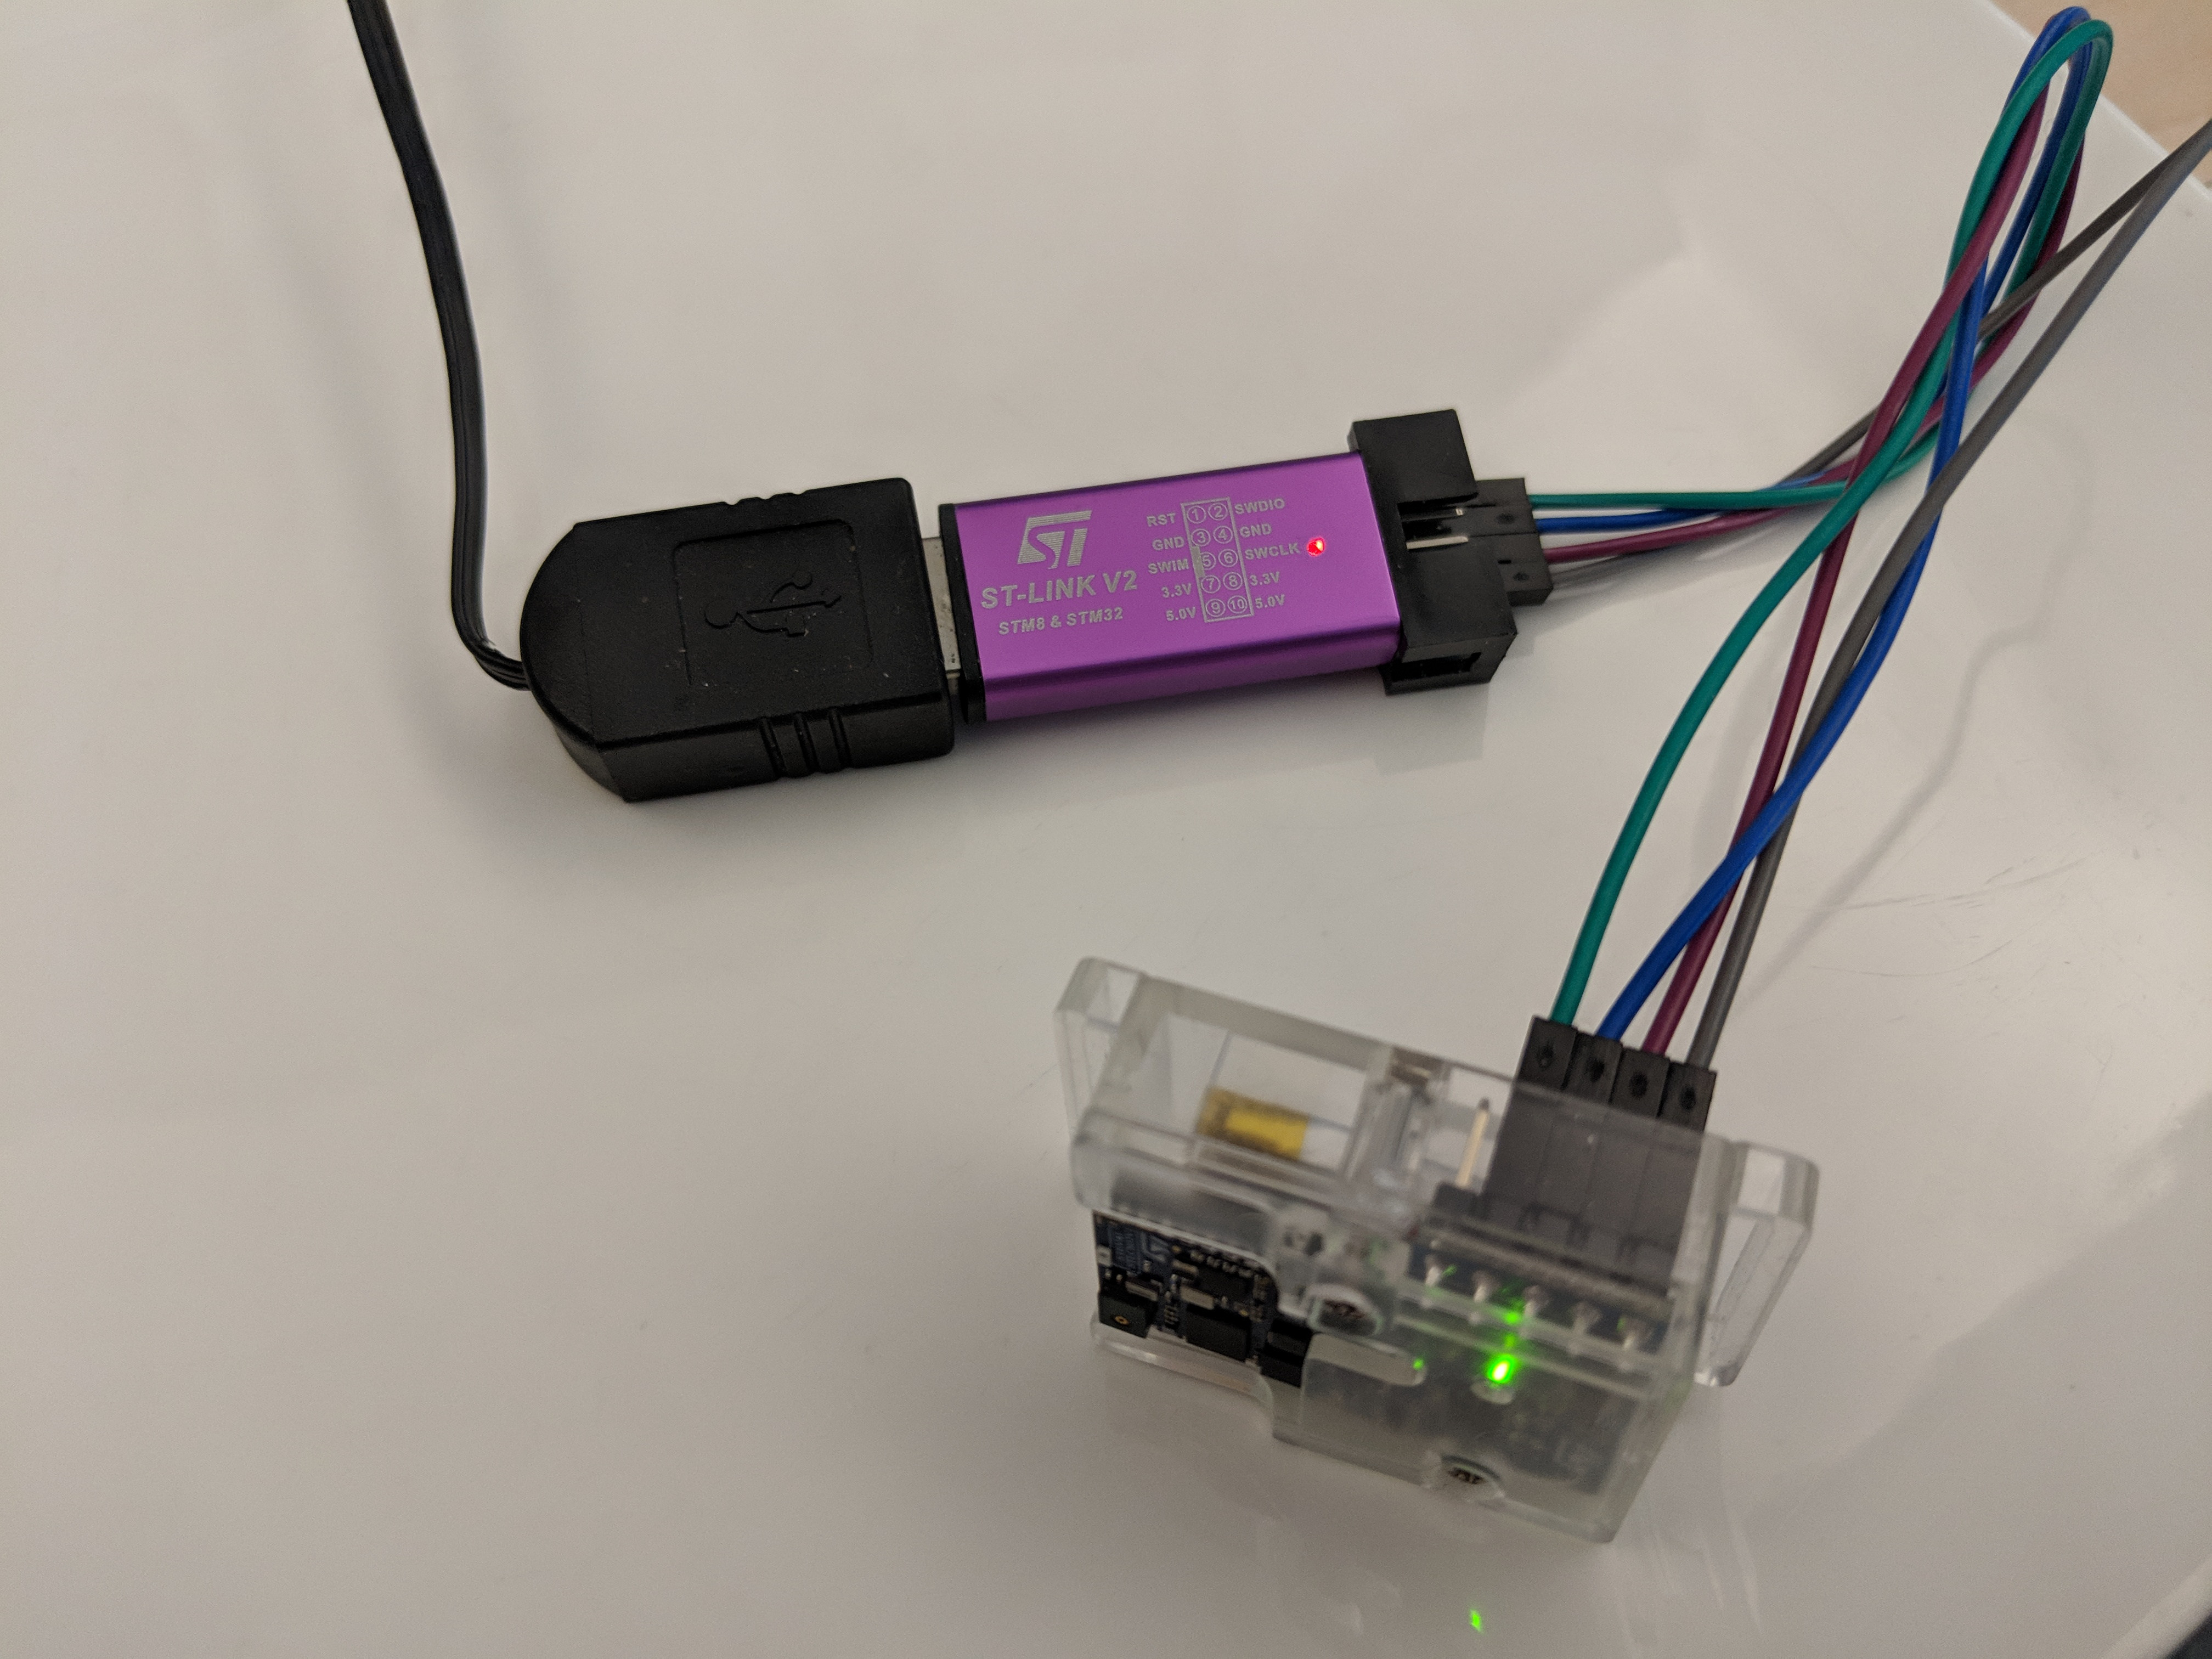
\includegraphics[scale=0.1]{STLinkV2.jpg}
\caption{STLinkV2 connected to a SensorTile}
\label{Figure:STLinkV2}
\end{figure}

\subsection{Examination phase one}
I had written some Ruby scripts a year or so ago that parse SVD
files. The SVD file contains all blocks, all the registers and all the
fields in the SoC in XML format. This includes symbolic names for all
the above and their numerical offsets, fields widths and base
addresses. AdaCore themselves uses the SVD files with a clever tool
svd2ada that emits a bunch of critical {.ads} files that are used by
the Ada\_Drivers\_Library to control the SoCs. Again, without SVD
files, I am sure even AdaCore would not have approached targets
without such automatic mapping. An SVD file entry for an L476's DAC
block might look like this:
{
\fontfamily{bera}\selectfont
\lstinputlisting{dac.xml}
}

My Ruby tools, svd2gdb and logs2dump both take an SVD file as an
argument, the first tool emits scripts that GDB uses to dump all SoC
blocks, the second takes the dumps and composes them into human
readable info. Lets see partial output of svd2gdb first for the DAC:

{
\fontfamily{bera}\selectfont
\lstinputlisting{dac.txt}
}

\clearpage
The partial resultant output from GDB after you run that script is:

{
\fontfamily{bera}\selectfont
\lstinputlisting{dac.dmp}
}

And the partial interpretation of the dump via log2dump:

{
\fontfamily{bera}\selectfont
\lstinputlisting{dac.output}
}

The scripts are on my GitHub. You can use them on any SVD file, they
are not ST specific so that makes them quite useful for the future I feel.

\url{https://github.com/morbos/ruby/tree/master/svd2gdb} and \url{https://github.com/morbos/ruby/tree/master/logs2dump}

\subsection{Examination phase two}
So this then allows us a window into a target SoC to see what
registers are set at the moment we halt the SoC in GDB. All we need do
is to source the GDB script and we then get 76 log files generated for
each of the blocks in the STM32L476. We then recompose those logs with
the benefit of the SVD file to put human readable structure back onto
the raw register reads. In this way, we now have a human readable
story on the state of the SoC at that moment. A small leap ahead
allows us to see that we can take a working SoC FW, stop it, dump its
state and then take the state of a non-working SoC FW, perform the
same state dump and then diff the two human readable output files,
where there are differences could be clues as to why the non-working
FW is indeed not working. I have used this technique on STM32s to
great effect accross a whole range of parts. I do encounter SVD file
bugs from time to time as I delve deeper into the designs. I repair
these errors always with the central tenet that the datasheet is the
arbiter for correct specifcation. Indeed as I have done these repairs,
that has always borne out. As I repair the SVD file, I refold it back
into the svd2ada {.ads} build. Now at the end of January, I now see ST
has updated their SVD files to v1.2. v1.2 adds much more detail to the
CPU. (MPU, systick etc). I believe I am still on v1.1 but still I did
not see some of the fixes I made so I think I will stay with v1.1 for
this project.  Bringing this back to the examination phase, ST
provides the ALLMEMS FW for SensorTile evaluation. Its a download from
ST's website and can be compiled with the free eclipse gcc based
toolchain. ST calls the toolchain, System Workbench. Projects
associated with that toolchain are in the SW4STM32 dirs. Once the
ALLMEMS elf file is built, it can be flashed on the SensorTile. Using
gdb as I mention, we can stop the target and take a state dump of
it. This is becomes the gold standard for what I needed to achieve in
my Ada bringup. For more advanced study, some mods were made to the
ALLMEMS FW to make a ring buffer. At certain points in the FW, bytes
are logged into the ring and they get saved to the disk in a similar
fashion as the raw register dumps. This particular ring is used for
outgoing BLE packet data and incoming interrupt data. Another Ruby
script was crafted, this one has initimate knowledge of the BLE API
call structure and can reassemble the packets sent to and fro. Another
important tool is the ST CubeMX Windows software. It will allow
creation of a project that is tied to a particular SoC or board. The
SensorTile is not one of the boards selectable but the SoC, the
STM32L476 is. We create a project using that SoC and begin to setup
the clocks. Also we can use the CubeMX to examine pin alternate
functions. It can also generate C code but I did not use that option
for this target.
\subsection{Preliminaries}
Armed with the tools some steps can be taken. First is to begin an
Ada\_Drivers\_Library for the L476. To begin, we copy over the
L432. The L432, whilst complete enough last year for a simple
challenge is not robust enough for SensorTile work as will be
discovered. So we have a library, change the flash and ram specs,
modify OpenOCD to for the L476, we can build a small
program, tryL476. Failing to reach main, we begin the task of
asymptoting to the init seq ALLMEMS uses. We start to narrow down PLL
differences and back patch those into the setup\_pll function. This
continues until we finally reach main as by then slowly but surely the
diffs were ironed out. SensorTile RCC clocking is different from a lot
of STM32 platforms I have used. It uses the on chip oscillator. That
on chip oscillator (MSI) can reach 48Mhz via factory tuned constants that
are loaded up at PoR. Actually, I had a bug in my code that assumed
the MSI was 4Mhz (factory default) for the SensorTile. A close
examination of the diffs however showed that the ALLMEMS FW bumped
that MSI clock to 48Mhz. Anyway, with the diffs, its all pretty
straightforwards to catch these types of discrepancies.
\subsection{CM4F Memory Protection Unit (MPU)}
I should also mention I run the CM4F on the STM32L476 like a police state. That
means I have numerous code/data and device regions set in the MPU. I set all ram to
eXecute Never (XN). Each region is sized only as big as it needs to be
to allow normal access.
\begin{table}[h]
\begin{tabular}{|l|l|l|l|l|}
\hline
Region \# & Address & Size & Attributes & Comment\\ \hline
0 & 16\#00000000\# & 4GB & No access & Lowest pri faultall region\\ \hline
1 & 16\#08000000\# & 1M & Read Only & Flash memory\\ \hline
2 & 16\#20000000\# & 128K & Full access, XN & SRAM1 (its physically 96K)\\ \hline
3 & 16\#10000000\# & 32K & Full access, XN & SRAM2 (used by logger curr)\\ \hline
4 & 16\#40000000\# & 256M & Device space & STM32 periphs\\ \hline
5 & 16\#50000000\# & 512K & Device space & STM32 periphs cont\\ \hline
6 & 16\#E0000000\# & 64K & Device space & ARM periphs\\ \hline
7 & 16\#1FFF0000\# & 64K & Device space & STM32 system space\\ \hline
\end{tabular}
\end{table}

Wandering outside of the MPU regions denoted above will place you in the
fault handler. To Ada's great credit, you have to try very hard to get
a compiling program to enter an ARM fault handler, normally you will
be in the 'last chance handler' long before a bad access has a chance
to present itself. Not so with C, I routinely enter fault handlers
during development when the MPU is hardened as I have done here (which
is where the fault handler shown below came from). The fault handler
has been modified to give a little more colour to the nature of the
fault. Observe only r0-r3 are used as the real r0-r3 are stacked at
fault time. There is also another function 'hang' that has the same
treatment.

{
\fontfamily{bera}\selectfont
\lstinputlisting{fault.S}
}

\subsection{First FW}
So we have a library and we can get to main. The first order of the
day was to talk to a sensor. I decided to start with the LPS22HB
pressure sensor. The work began with a generic driver for it. Seems
all pretty straightforwards. One difference was that ST was using SPI
3-wire mode. All the previous SPI sensors I have used were 4-wire. 3-wire
is a bit like I2C in that, like the SDA line, one of the communication
wires needs to be turned around on a read. So the Ada setup for this
is a bit different:

{
\fontfamily{bera}\selectfont
\lstinputlisting{3wire.adb}
}

So now, with suitable initialization we can try to talk to the
sensor. Perhaps not surprisingly, it did not work. As I mentioned
earlier in this document, no probing is possible on this
SensorTile. Thus we are presented with a puzzle, how to diagnose balky
communication on this new (to me) 3-wire SPI connection? So now, I
will reveal another method I used. I have a webpage
\href{http://hrrzi.com/2018/02/the-bluepill.html}{Bluepill+}, where I show how I
performed a brain transplant on a sub-\$2 Bluepill board by
replacing its STM32F103C8 (a 10yo CM3 design btw) with a modern pin
compatible STM32L443CC SoC. (\textbf{Massive} hat tip to ST Microelectronics
for supporting a 10yo footprint!). Now, the STM32L443CC is a close
cousin of the STM32L476 and shares a great deal of commonality. A
Bluepill board is the opposite of a SensorTile, 1) its large (relative
to a SensorTile) 2) all the SoC pads come out to easy to connect
\SI{0.1}{\inchQ} centre pins.

\begin{figure}[H] % bluepillplus
\centering
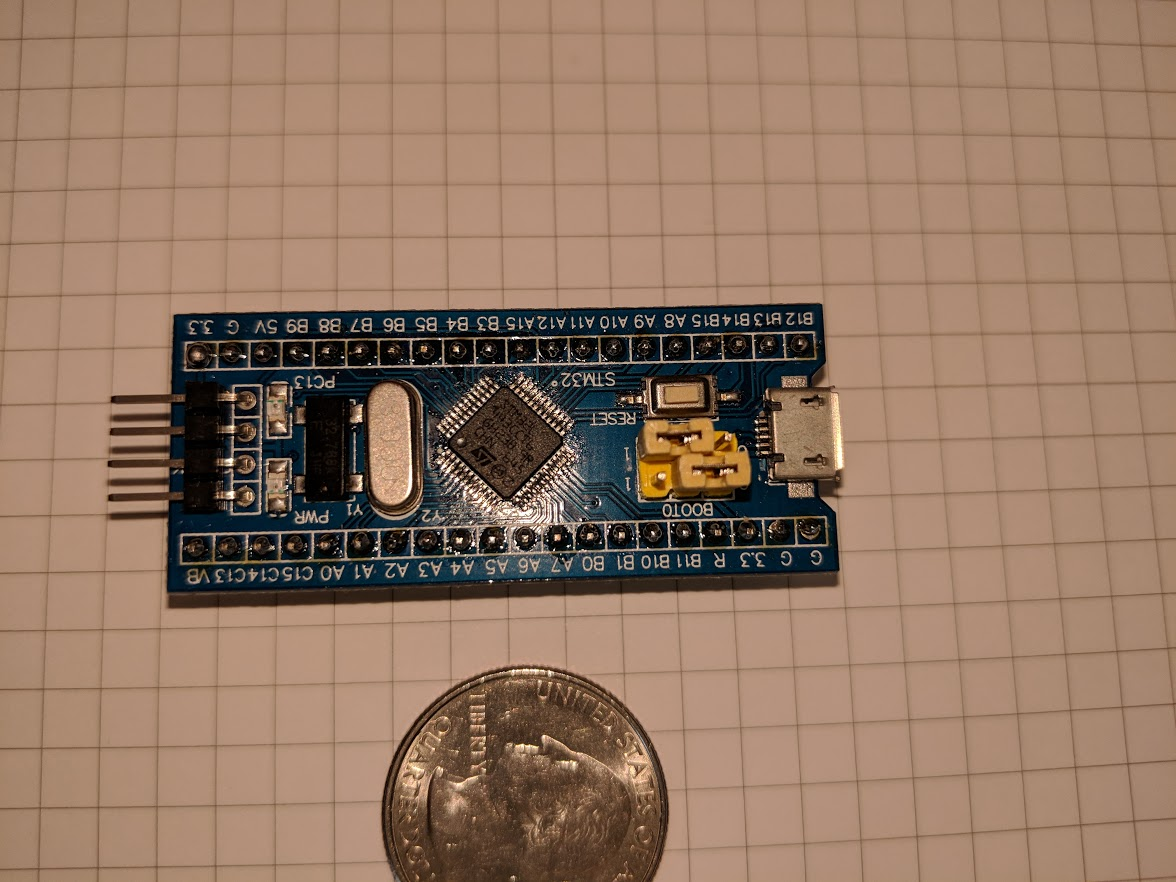
\includegraphics[scale=0.5]{bluepillplus.jpg}
\caption{A Bluepill+, created via an SoC swap}
\label{Figure:Bluepill+}
\end{figure}

Perhaps you see where I am going with this? We can take an ST sensor
(like the LIS3DSH) and connect it to the STM32L443 using wires, then
we can try the 3-wire SPI code with that sensor and shake down where
in the library the issue is. Since its a bare wired physical
connection, a Saleae analyzer can be used to diagnose the protocol.
Once the issue with the library is sorted out for the L443
we move the change to the L476 library. Via a rebuild, we retry the
pressure sensor and magically, it now works. Subsequently, pressure
readings were pulled out and the numbers seemed OK.

Much later I had another bug with 3-wire that was a lot harder to
find. Basically, the accelerometer/gyroscope and magnetometer readings
would become erroneous. First step was to compare a diff of ST's
ALLMEMS FW vs mine. After giving that a good study, I noticed the
overrun bit was set in my dump of the SPI2 status reg. This was a good
clue and I followed up using the {Bluepill+} technique, I was able to
analyze that at the fast baud rate that the SensorTile was using, it
was possible to get an overrun. 3-wire SPI is a bit odd, all is good
for writes to the slave, its when reads happen that the fun
begins. The write is a bit like 4-wire SPI then, you disable the SPI
and restart it in 3-wire mode. Once you do that, the SPI block will
emit a \textbf{continuous} stream of clocks out to the slave, the
slave, also configured as a 3-wire device accepts this and dutifully
begins to emit bytes on the wire, because the stream of clocks is
continuous, you have to shut the valve off once you get your
data. Unfortunately the timing of that can be tricky and invariably
once in a while another byte is clocked into the fifo. Subsequent
reads, not expecting, this can go out of sync. The fix in the library
was as so:

{
\fontfamily{bera}\selectfont
\lstinputlisting{bider.adb}
}

\subsection{Moving on}
Now that we can talk to one SPI 3-wire sensor, we can talk to
more. There are 3 SPI sensors in a SensorTile. Each has its own chip
select. So the next FW was one to enumerate all the sensors by
checking their ID's. Register 16\#0F\# in most ST sensors is call a
WHO\_AM\_I register and returns a unique code for that sensor
family. Once that FW was ready, we could verify that all the sensors
were present.
\section{BLE (or the elephant in the room)}
Well, one can keep probing sensors all you like but ultimately, to be
useful and perhaps the raison d'etre for this project entry was to get
ST's BLE chip working with Ada as a pure Ada driver, not a
hybrid. By the way, I tried a hybid for a week or so, basically
linking Ada vs ALLMEMS C FW. I got some OK results but the entire
structure of that was impure and not at all where I wanted to go. You
see, ST's BLE, as a single chip peripheral, is just a stepping
stone. In March of 2019, ST will world release the STM32WB. Basically
its an STM32L4 + BlueNRG-MS, some slight changes since both IPs are
on the WBs SoC they don't use SPI but an interprocessor communication
channel. So if we can overcome the elephant in the room, we will have
a BLE stack that can move easily over to the new single chip design
next year. That is the ultimate goal. The SensorTile is a method to
get us there.
\subsection{BLE first steps}
Its pretty straightforwards to get the BlueNRG-MS plumbed over to the
STM32L476 we have all been connecting 4-wire SPIs to STM32s for a
while now, this one is no different, initially. Relatively quickly,
one finds that the BlueNRG-MS uses the interrupt line to alert the
STM32L476 that packet data is waiting. So, we need to plumb over the
interrupt line and get a handler in place at the correct
EXTI9\_5\_Interrupt. Once again, the diff technique worked wonders as
its easy to make sure all the GPIO's are right and the NVIC is set to
take the interrupt. Now, a BlueNRG-MS will not spontaneously begin
interrupt transmission, you need to get it initialised to start
that. I figured the first command I would go with was the one that
interrogates the revision and manufacturer info from the
BlueNRG-MS. This is officially where the rabbit hole begins. Just to
transmit that revision request and handle its reply requires BLE
outbound command processing, inbound command parsing, data structures
and a lot of other procedures and functions. Then the record is sent
with a reply pointer set to where the reply goes. Now the call to the
send is a blocking call and after the comand is sent, an interrupt
comes back with indication of a packet waiting (the response). How
packets are passed around in ST's BLE is via a doubly linked
list. They have a structure like this:

{
\fontfamily{bera}\selectfont
\lstinputlisting[language=C]{st_list.c}
}

That structure relies on the fact that they can process the linked
list separate from the payload. They tack the payload after the
currentNode declaration above. This allows them to have arbritrary
elements after the linked list record and write the linked list code
without any knowledge of the dataBuff element for example.

In Ada, we cannot partially specify a record and then promise to fill
it in later when we know what will follow. So in my implementation of
the doubly linked list I made it a generic where the element that
follows the linked list record is a type that is passed in. In this
way, we cleanly pass the payload when we instantiate the generic as
so:

{
\fontfamily{bera}\selectfont
\lstinputlisting{gen_list.ads}
}

I am embarrassed to reveal it took a few weekends to get that doubly
linked generic to a point where it was usable. After a rather nasty
deletion bug it was finally ready for use. You need only five 128byte
packet buffers to make this BLE stack work. The linked list data
structure is critical to all phases of packet processing in the
stack. I feel the time was well spent as once it was created, we now
had a solid data structure that was 100\% Ada and able to handle the
packet flow.

Now back to the revision query. So after we climb out of data
structure prep, next is composing the query. There is a certain format
that BLE (and perhaps BT itself) use comprising ogf and ocf codes,
these two fields end up being composed into a 16bit field. The two
numbers seem to be the division of the API request and the actual code
within the division. The divisions are formed by a 6 bit OGF value and
a 10bit OCF code. For the revision number you end up with this:

{
\fontfamily{bera}\selectfont
\lstinputlisting{ocfogf.ads}
}

Which makes a req of 16\#1001\# after sliding the OGF value up to the
top 6 bits.

Here is a partial output from the Ruby script analyze.rb that I
mentioned further up that helped to parse the raw gdb ring buffer
memory to recreate the sequence of calls to and from the
BlueNRG-MS. Observe the results at the top to the revision query. Note
that 0030 is ST's hex Bluetooth manufacturer id.

{
\fontfamily{bera}\selectfont
\lstinputlisting{pktlog.txt}
}

The analyze.rb script
is also on my GitHub:
\url{https://github.com/morbos/ruby/tree/master/analyze}

Just issuing a packet is not a sure thing. ST has an odd SPI retry
that continuously keeps transmitting the pkt until the reply back is
correct. One thing to note here on SPI communication to the BlueNRG-MS
is that its transmit\_receive, so we expect a reply the moment we send
data. Sometimes the BlueNRG-MS will push back with a not ready code so
a retransmit is required.

{
\fontfamily{bera}\selectfont
\lstinputlisting{halwrite.adb}
}
\subsection{HCI\_Isr}
To get the replies back, a routine HCI\_Isr is used. This is the
procedure that gets called once the EXTI line for the BlueNRG-MS
device asserts. Below I attach the handler. It is a critical item for
getting BLE going. When the EXTI asserts it loops whilst BLE data is
ready. There is a read packet pool, its full when there are N packets
ready to be allocated and empty when all packets are busy. In the case
its busy, the handler just acks the interrupt but doesn't take the
packet. In the other case, it takes the packet and makes some
decisions about what queue to attach it to based on validity and len
of the payload, if all is ok, it goes on the RxQueue otherwise, length
zero or invalid, the buffer gets recycled back into the free pool. HCI\_Isr
also is called from a number of non-interrupt contexts. In each case,
its to move along a blocking call by clearing out BLE traffic from the
BlueNRG-MS. At some point in the future, I would like to revisit this
software architecture and restructure it with threads. Ideally,
HCI\_SendReq could be linked with a thread who sleeps on a suspension
object which is set when a suitable BLE packet arrives. In this way,
the HCI\_Isr can be just that and not a general purpose function to be
called almost in a polled fashion.

{
\fontfamily{bera}\selectfont
\lstinputlisting{hciisr.adb}
}

\subsection{BLE setup}
Intialization of the BlueNRG-MS after the revision query finishes
follows. There are some messages that need to be sent to get the radio
up and able to transmit with a specified power etc. Also, one main
activity is the setup of the characteristics. You first need to create
a server handle. Off of that server handle, you then prepare as many
characteristics as your application needs. These char APIs have UIDs
that uniquely identify the service being requested or provided to the
other side. For example, when ALLMEMS creates its UIDs to communicate
with the iOS or Android app, there is an agreement between both sides
as to what those UIDs are as they identify the functionality on that
char channel. Let's take the accelometer/gyroscope/magnetometer as an
example. We want to send 3D data from each sensor. Each data element
is 16bits. So this means we need to send at least 18 bytes. Each
characteristic over to the mobile app also prepends 2 byte timestamp
in milliseconds to the packet. So 20 bytes makes for the full size.

{
\fontfamily{bera}\selectfont
\lstinputlisting{accgyromag.adb}
}

So that is the declaration for just one characteristic. Fully, there
are 16 characteristics declared. For our Ada port of BLE, only
environmental, AccGyroMag and Battery are supported. There are others
like AccEvent that use the special features of the MEMs sensors to
report things like gestures etc. Also we don't handle the sensor
fusion code. ST has a binary blob in ALLMEMS that is full of vector
dsp code to do sensor fusion. My goal was not a perfect workalike for
all these characteristics but to get a useful working subset over
BLE and to demonstrate that. Using the code stack built, it will be
possible to tailor all types of characteristics to host
requirements. As an example, I was able to get a Raspberry Pi3 via its
on board BLE stack to communicate with a SensorTile and extract the
acc/gyro/mag data.

{
\fontfamily{bera}\selectfont
\lstinputlisting{scan.py}
}

When run on my RPi3 you see the results below. Observe in the data shown,
Az is \textasciitilde{1000}, this is 1000mg or 1g. The first field is the timestamp in
8ms per tick. I tipped the sensor to show changing data.

{
\fontfamily{bera}\selectfont
\lstinputlisting{blue.txt}
}

So this shows we are device agnostic and are not bound to
communicating only with ST BLE solutions. Lots of possibilities for
sensor and data connection are possible here. Now we have Ada running
the communication its really a blank slate to be filled however you
like.

\section{Source tree}
\dirtree{%
.1 sensortile.
.2 src.
.3 comm.
.4 bt.
.5 hci.
.6 controller.
.5 utils.
.3 sensors.
.4 components.
.3 audio.
.2 doc.
.2 openocd.
.2 SVD.
}


All the BLE related hw and sw setup is in comm and below. The sensors dir has
the sensors.adx files which instantiate all the sensors in the
directory. Audio is exclusively for the client board which has the
PCM1774 codec + 3.5mm jack.
\subsection{Two board flavors from one source tree}
So an interesting question arises as to how the same source tree can
support server BLE and client BLE. Given the SensorTiles are identical
and only the carrier boards differ with respect to the complement of
on board sensors. All carrier board sensing is done via I2C3. If you
interrogate an I2C sensor and no-one is there to pick up the phone,
Ada\_Drivers\_Library will summarily raise a Program\_Error. So we can
use this to find out what board we are talking to. HTS and GG point to
the humidity/temp and gas gauge (battery) sensors respectively. Those two
parts are only on the client. The client board has the PCM1774 codec
part and no need for battery monitoring etc:

{
\fontfamily{bera}\selectfont
\lstinputlisting{except.adb}
}

The beauty of that solution I feel is it captures precisely what I
want between the server and the client board differences.

\subsection{Ada tasking}
Part of the source is a task. ST's ALLMEMS FW has an
\textbf{elaborate} use of TIM1's capture and compare regs to produce
timing ranges for the sensor packets. There is periodicity for each
characteristic to the host, they select this via having each of the
characteristics derated to the correct time they want via CC
channels. There are four CC channels and they are tricky to setup and
serve from interrupt context. Rather than descend down that rabbit
hole I took a different way. For each characteristic you enable, it
sets one timer up with the periodicity that char needs. Once the
interrupt arrives on the timer, a suspension object is set that
triggers a task that serves the activity. A bitvector reflects which
char is active.

{
\fontfamily{bera}\selectfont
\lstinputlisting{task.adb}
}

That task is triggered by incoming Timer\_4 ticks as so (Timer\_2 is used
for the millisecond count (prob could have dipped into the raw SYSTICK
value for that but that seemed a bit too hacky even for me)).

{
\fontfamily{bera}\selectfont
\lstinputlisting{irq.adb}
}

There is also another task used only by the client. Its for
scanning. I have two server SensorTiles and each has a different
addr. Rather than hackily continue to change the src whenever I wanted
to use one or the other its possible to scan for the server. There is a
call Aci\_Gap\_Start\_General\_Discovery\_Proc that will begin
scanning for a programmed interval. The results come in via interrupt
callbacks. The task has a state machine that waits for the scan to
finish and then to parse the result. If there was a match, then a
connection is made. The name the client looks for is: \textbf{MkAda S}
for Make with Ada Server. There is some interesting filtration in the
isr callback that has to dig into the advertising results and search
for an AD\_TYPE\_COMPLETE\_LOCAL\_NAME and once we see that, we check
the name for the previously mentioned string. If a match was seen, the
task is apprised and it then starts up the connection.
\section{The demos}
Its a bit of a challenge to demo a networking stack. A network is just
one of those things that we all know needs to exist but seldom need to
peer inside to see a bunch of cables or antennas 'doing their
thing'. At my day job, making wifi SoCs, to demo wifi, invariably there
are 4k streams being transmitted and received over wifi. At least
there you see a tangible result from the smooth delivery of packets
through the air. For this case, the SensorTile, I have chosen two
demos.
\subsection{App: ST BLE}
ST provides a free downloadable app 'ST BLE Sensor' for iOS and
Android. This app is a one stop for ST's BLE offerings and as such has
more features than we need to demo BLE connectivity. For my server
SensorTile I present 3 main activities.
\begin{table}[h]
\begin{tabular}{|l|l|}
\hline
Activity   & Description\\ \hline
Environment & Temp1\&2, pressure, humidity \\ \hline
Battery & State of charge with current \& voltage\\ \hline
MEMS & Acceleration Gyroscope \& Magnetometer\\ \hline
\end{tabular}
\end{table}

Here are some screen captures of the activities via the ST BLE app on
the authors phone.

\begin{figure}[H] % environment
\centering
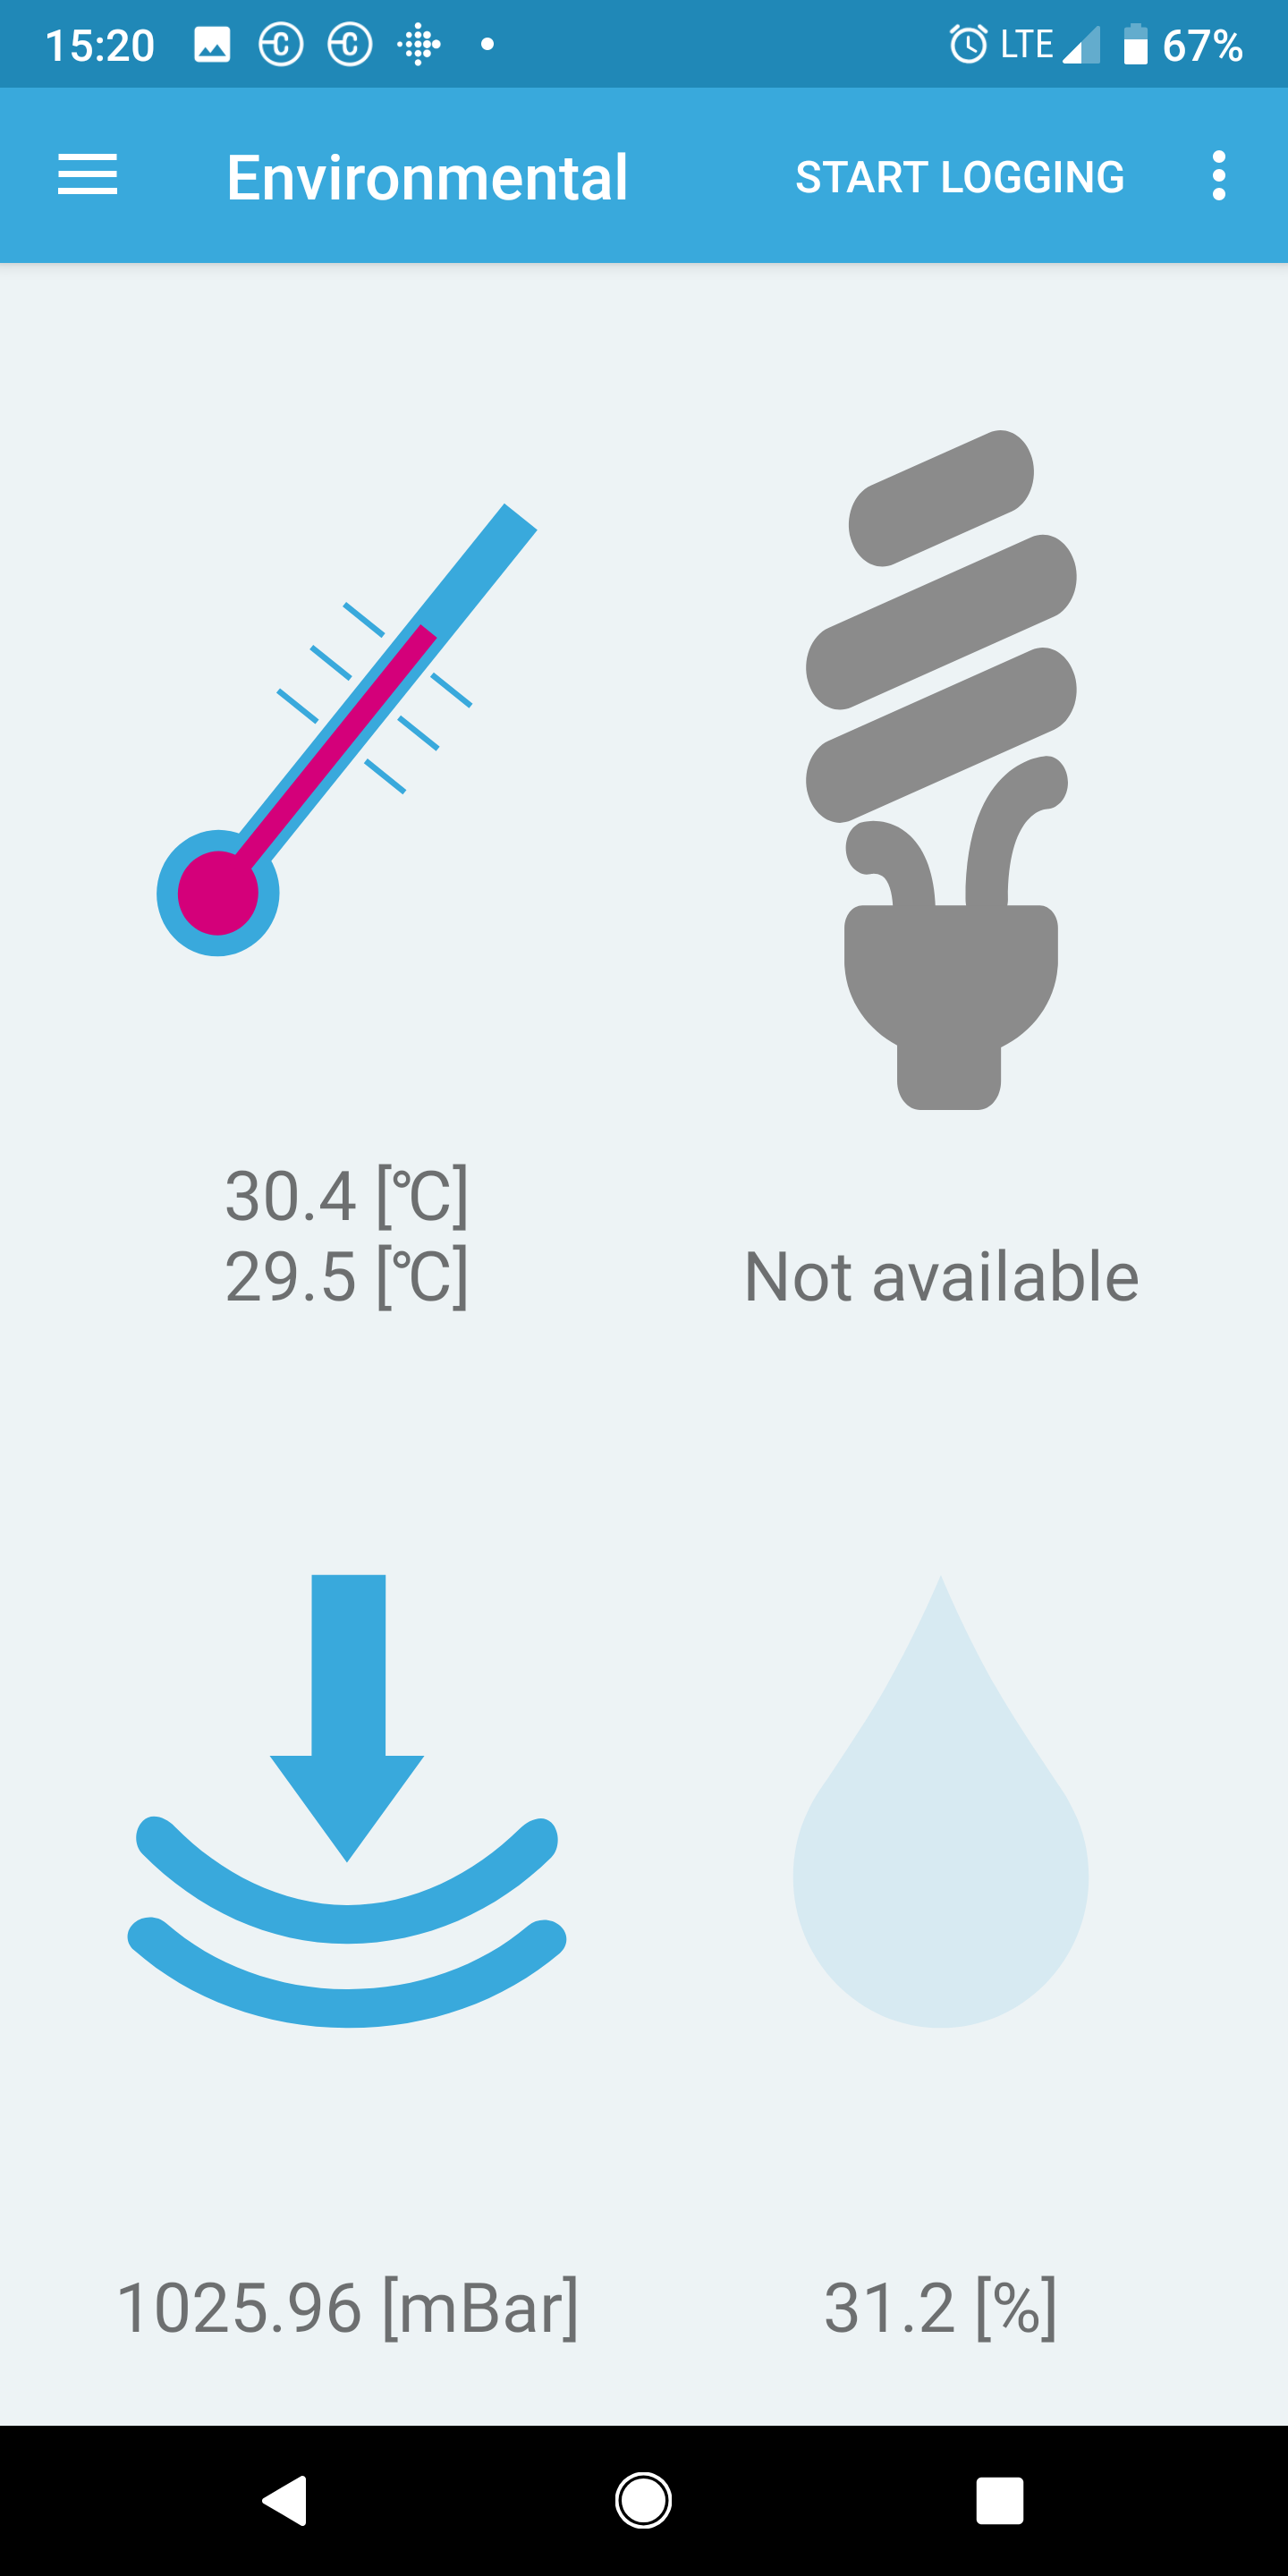
\includegraphics[scale=0.3]{environmental.png}
\caption{The environmental activity.}
\label{Figure: Environment}
\end{figure}

\begin{figure}[H] % battery
\centering
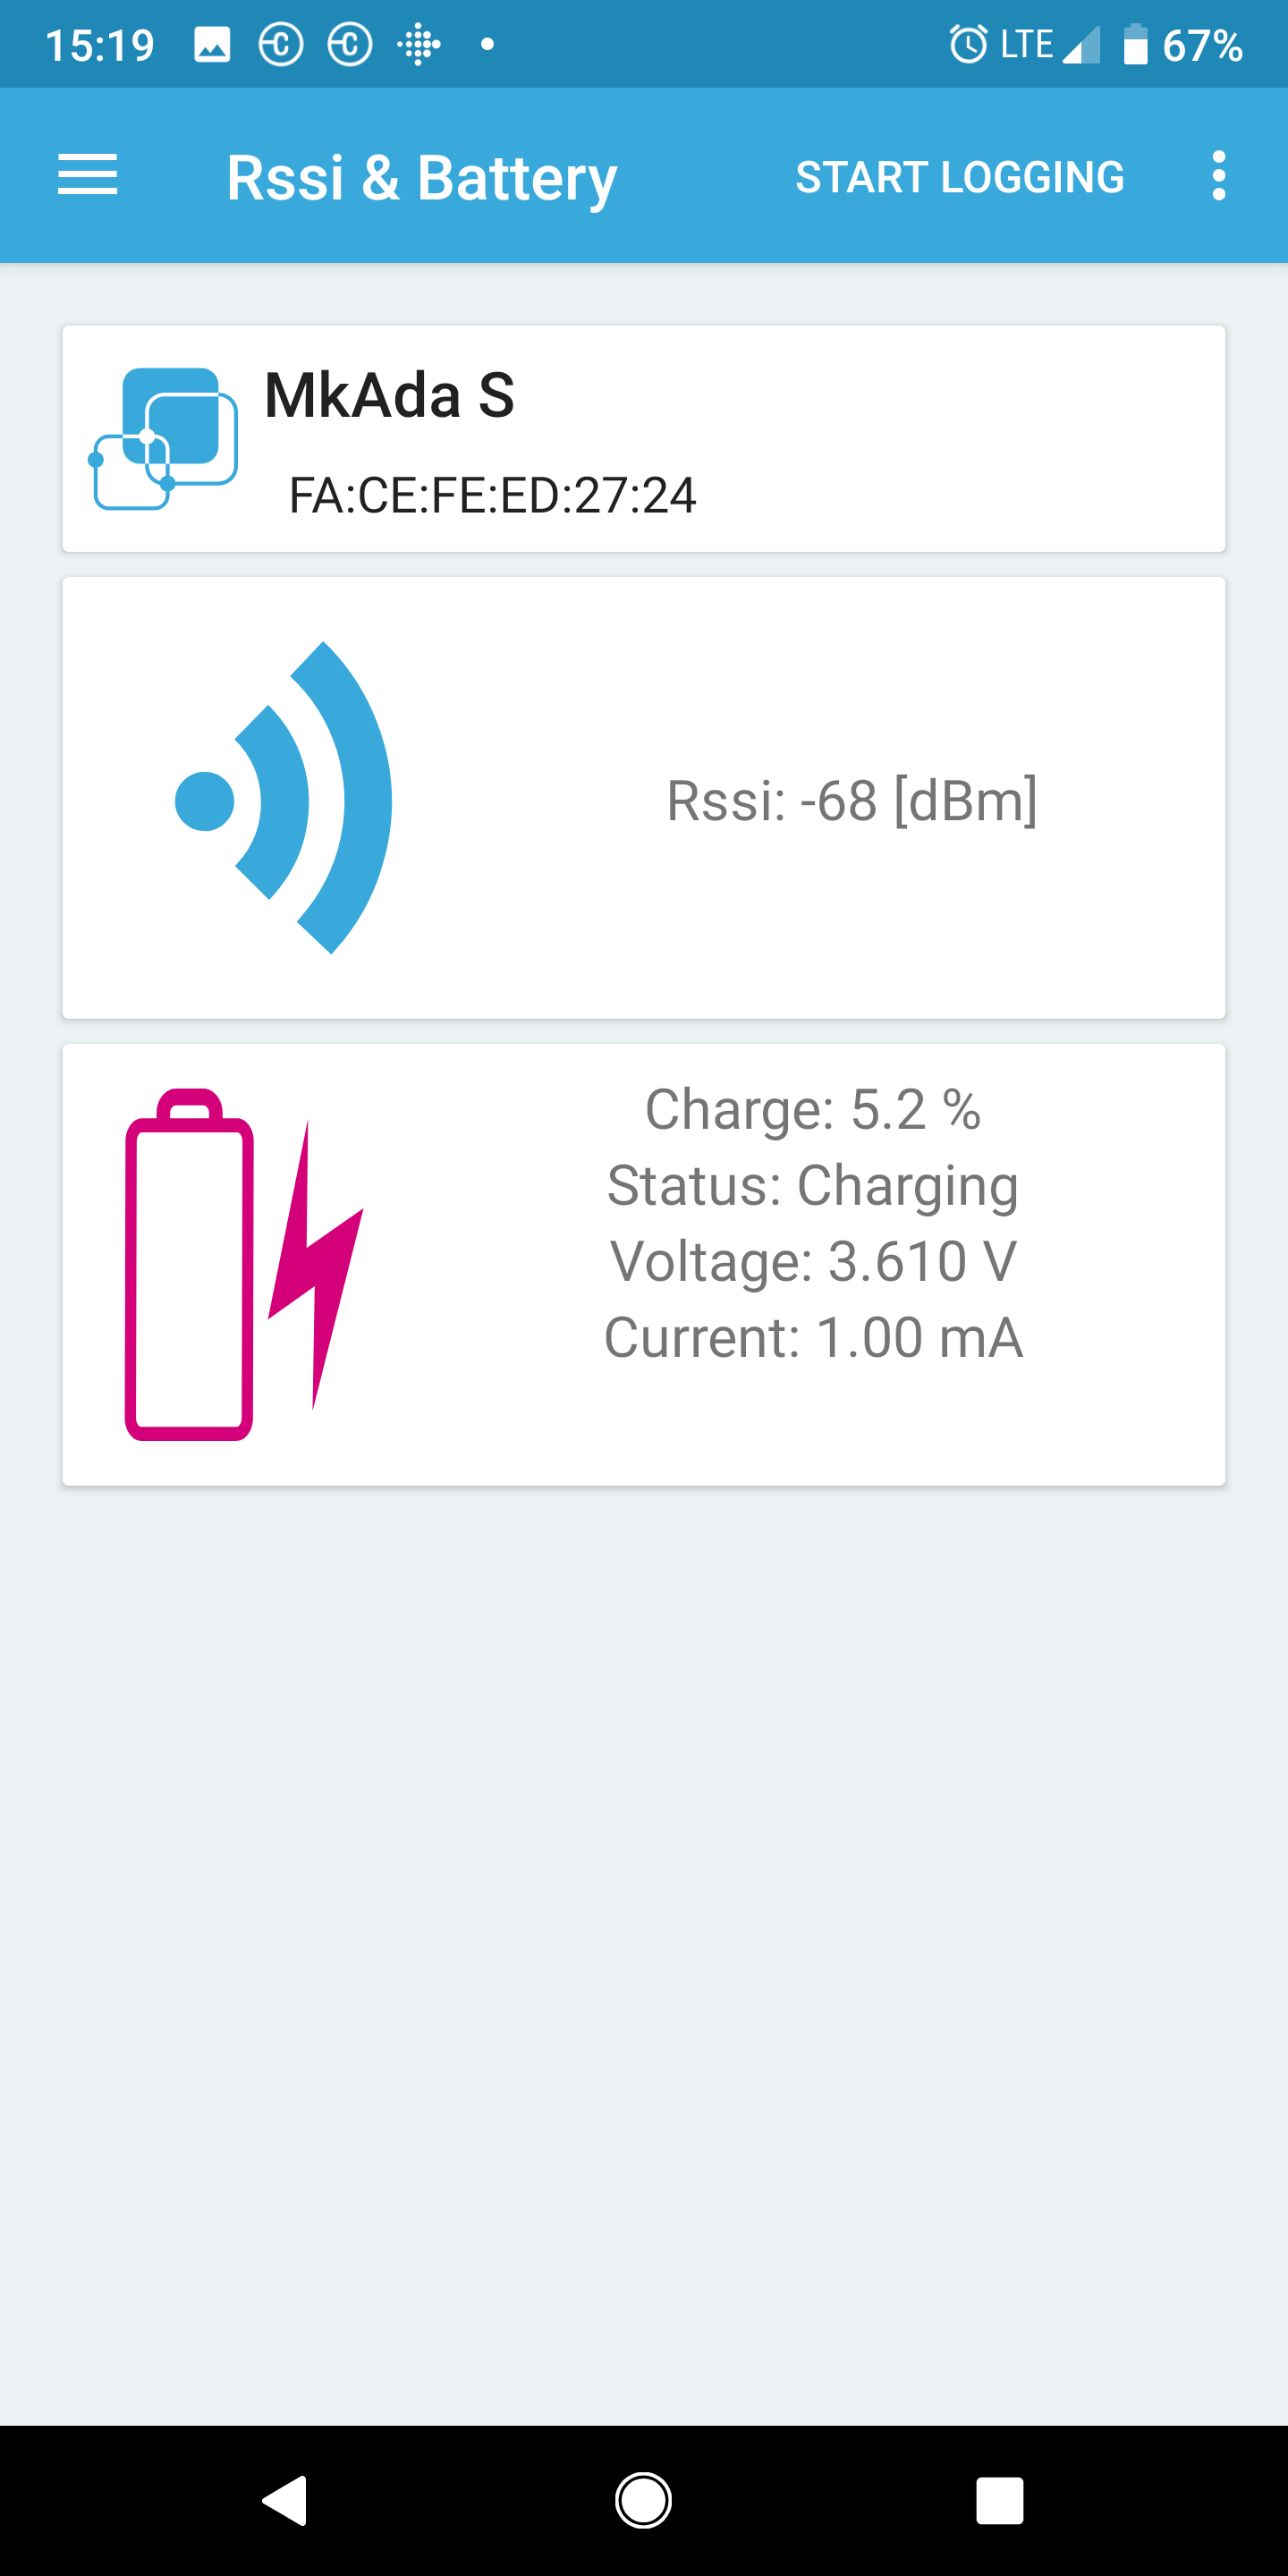
\includegraphics[scale=0.3]{battery.png}
\caption{The battery activity.}
\label{Figure: Battery}
\end{figure}

\begin{figure}[H] % accel
\centering
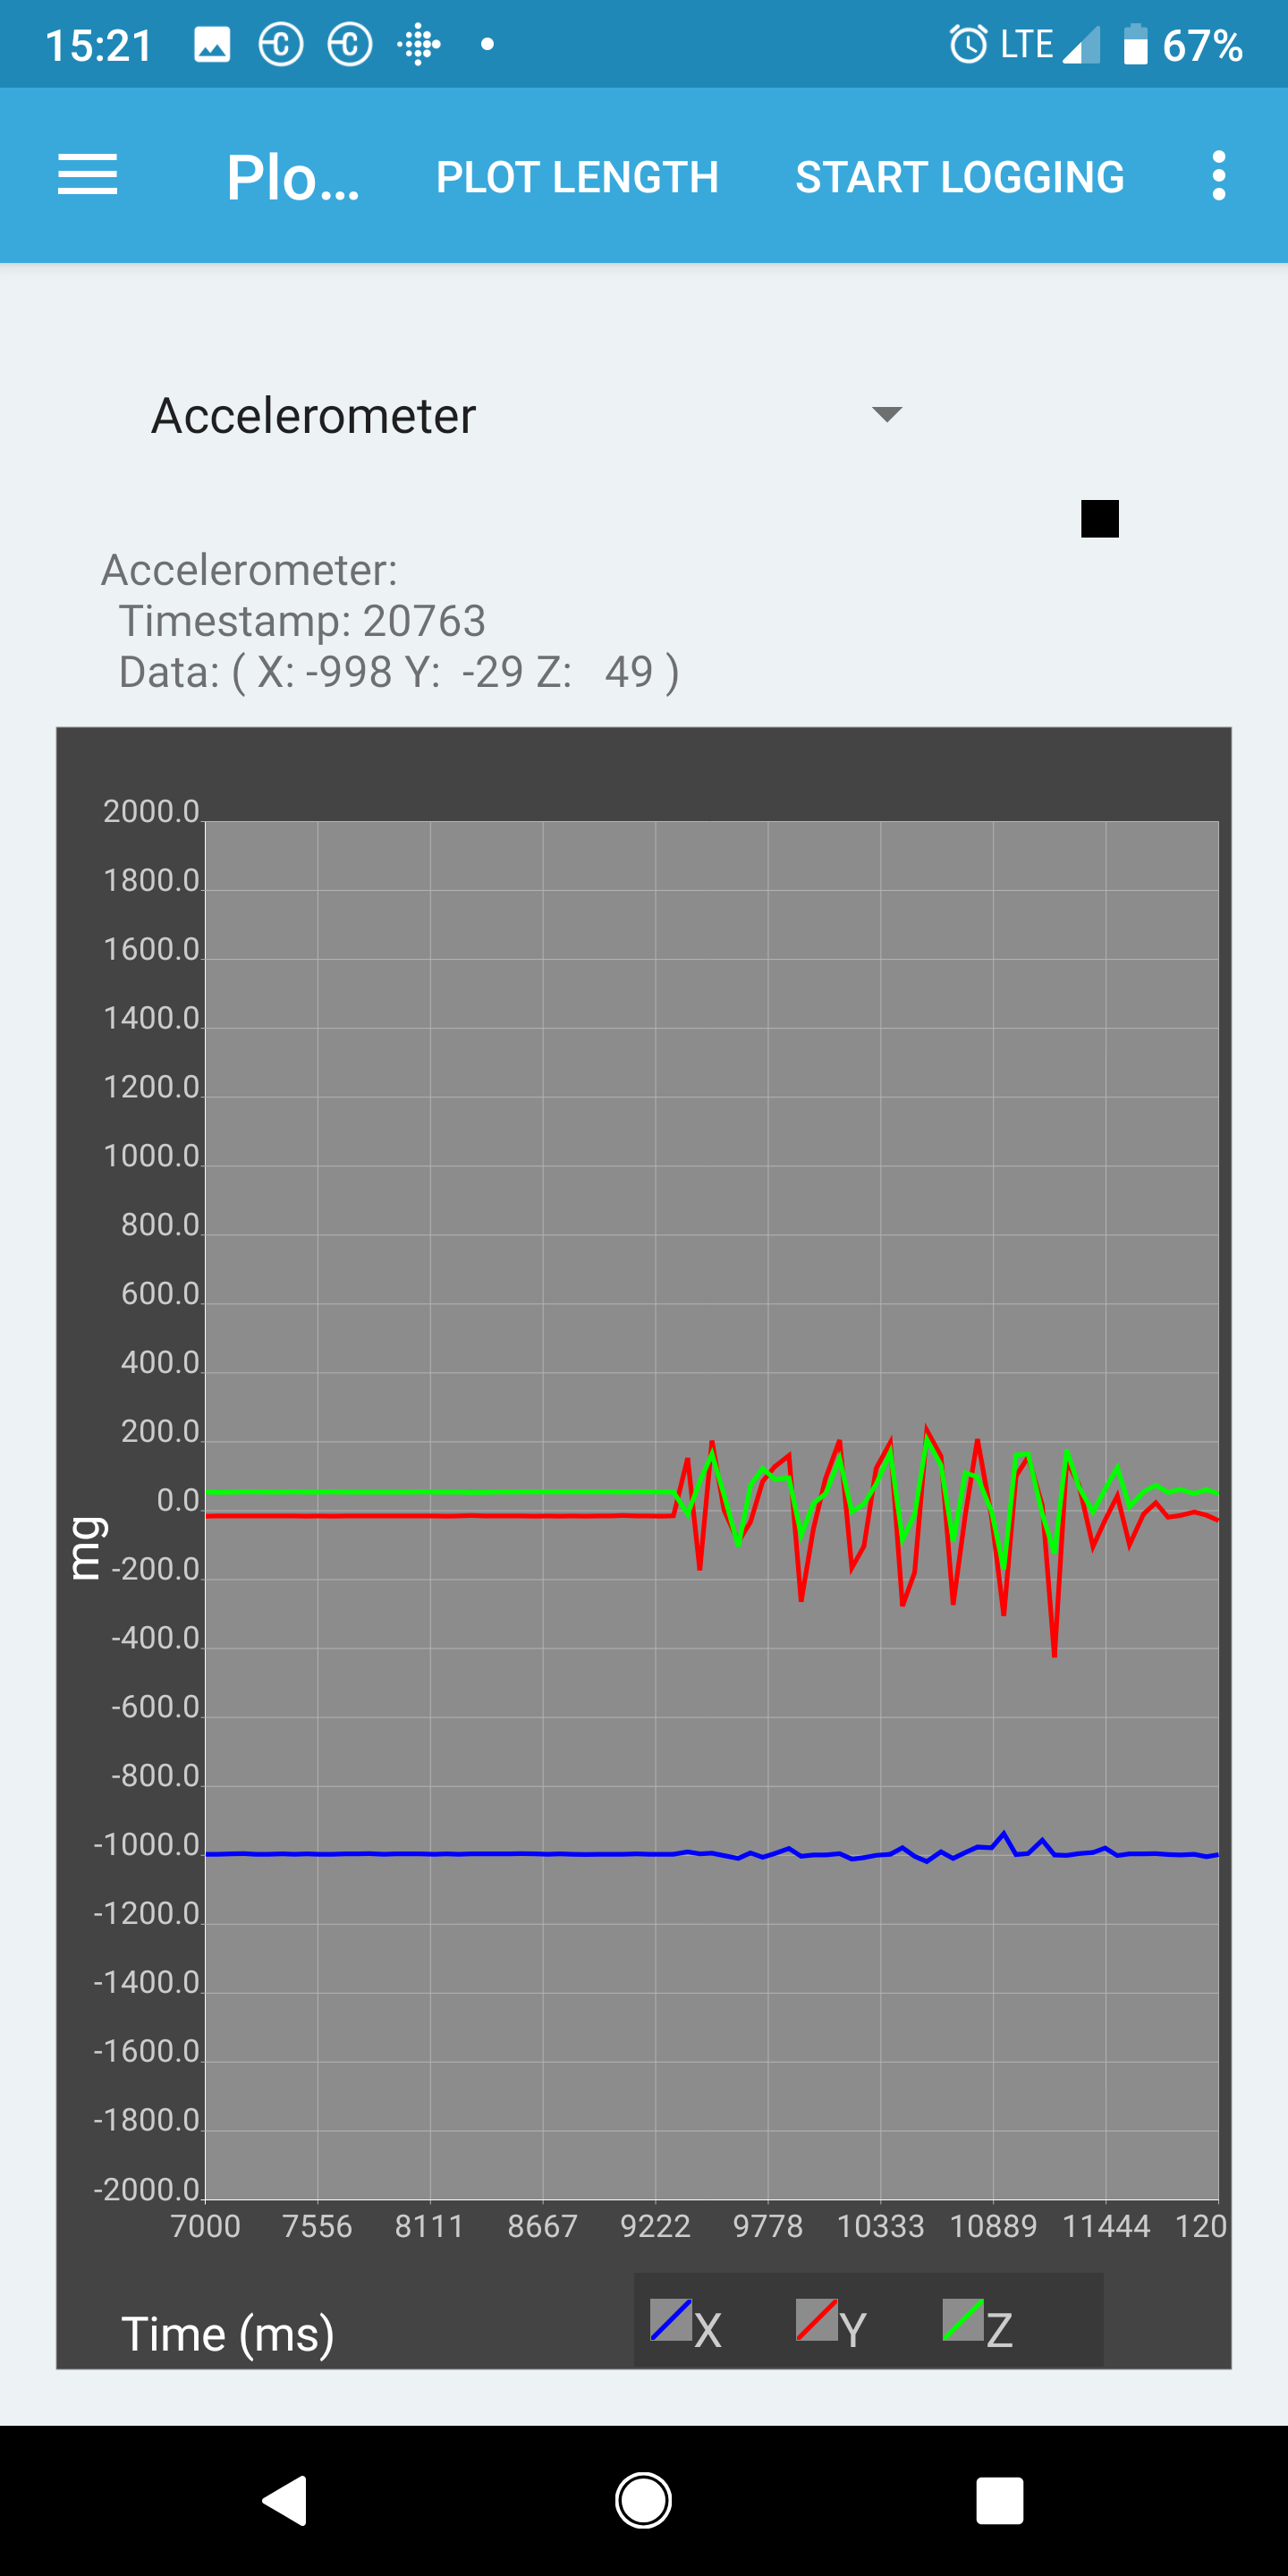
\includegraphics[scale=0.3]{accel.png}
\caption{Accelerometer plot}
\label{Figure: Accelerometer}
\end{figure}

Also there is a video that shows how these activities interact with the
server SensorTile.

\subsection{AdaTheremin}
This was a slog. First, someone told me that BLE chips could not be
both a client and server. That is wrong but it conditioned my thoughts
for a time. I had an idea that it would be cool if a SensorTile server
could send its data to a RaspberryPi and via its 3.5mm jack, emit
tones in sympathy to the motion of the users hand, all transmitted
over a BLE connection. This idea sat there whilst I worked on the
server and network bringup. At some point, looking at the larger
cradle, I was thinking it would be great if the SensorTile there could
act as a client to the server since there already is an audio dac with
3.5mm connector on the cradle. I pulled down some BlueNRG-MS demoes
from ST and one of them was a client-server example. It took some work
as like all things embeddded, nothing usually works right away. The
trick to get it to work was the goto strategy I use for debug, log the
BLE messages on client and server, filter via the Ruby analyze script
and try to isolate where issues appear. Actually another very useful
method is, the LED! First let me say that unlike other SoCs and
associated hookups, the one on the SensorTile is obscure. Yes, like
others a GPIO controls it, but to get the GPIO to work means enabling
another power domain in the SoC as its normally off. Once that was out
of the way, I had the client and server enable the LED when they were
connected. Finally, I had them both on once the comm bugs were worked
out and new functions needed for client operation were
in. Unfortunately, that told me something but not everything, namely
that they were connected but the server was not sending
anything. Finally, I assymetrically assigned the LEDs, when connected
the client would enable it but on the server, only when data was being
sent. This permitted me to locate a power up sequencing issue between
client and server. An LED is a valuable debugging tool, some folks
nowadays even PCM them to wiggle state out optically. Just after
saying this, I now have a port conflict once audio is introduced into
the picture. Audio on SD\_A also is on the LED pin (PG13), so if you
want audio out, you lose a GPIO that controls the LED. I should
mention at this stage that another relatively common occurance has
happened with my experience of embedded Ada development, namely that
the audio out worked almost first time. That meant, channel DMA (vs
streams used in F4, F7), SAI ported over from the
Ada\_Drivers\_Library for F7 and all the attendant RCC PLL enables for
SAI1 (and routing to SAI2). Plus the PCM1774 inititialization. I
expected to lose a week of debug on this to get it going. I had a good
bug that has a characteristic sign (no pun intended). Namely, use of
UInt16 for the samples when Integer\_16 was needed:

\begin{figure}[H] % scope
\centering
\includegraphics[scale=0.1]{scope.jpg}
\caption{Unsigned 16 bit output when Integer was needed}
\label{Figure:Scope}
\end{figure}

\subsection{Magnetic fields}
To achieve the AdaTheremin, some magnet work needs to take place. The
basic idea is a disc magnet from K-J Magnetics, the D83-N52, is used
to emit a field wherein the SensorTile can be used to detect it and
deduce its position in the field from the XYZ vector returned. Per
KJ's website, here is the field:

\begin{figure}[H] % D83
\centering
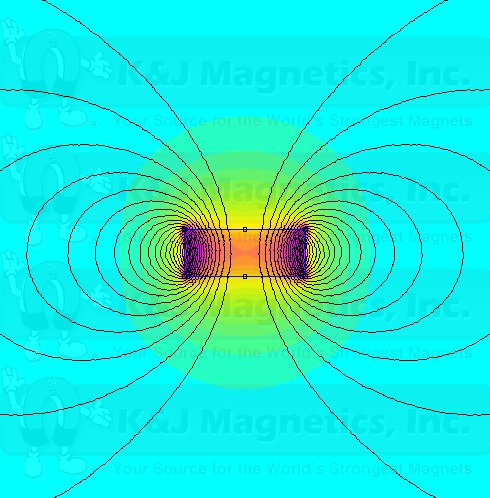
\includegraphics[scale=0.5]{D83-N52.png}
\caption{KJ Magnetics 2 dimensional field from a D83-N52 disc magnet}
\label{Figure:D83-N52}
\end{figure}

If you look at how a real Theremin works, there are two antennas. The
tall one on the right is for pitch. As your hand approaches that
antenna, the pitch rises. The flat loop antenna on the left is
controlled by the left hand to control amplitude. Touching the loop
produces zero amplitude going to progressively higher amplitude in
proportion to the players hand distance from the loop. For the
AdaTheremin a magniture is computed from the magnetometer's XYZ
vector. The force seen by the MEMs magnetometer is proportional to $1
/ distance^2$ so we map that force change as a pitch change.  The
force range change is translated to this frequency band: 100hz to
3hkz. In lieu of a left hand amplitude computation the angle of the
sensor to the horizontal plane in front of the magnet is translated
into the PCM1774 amplitude. If the sensor is tipped to the left the
amplitude is reduced and if tipped to the right, it advances to the
maximum amplitude.

\clearpage
\subsection{Audio generation}
This was another \textbf{major} diversion. At first blush, audio is a slam dunk,
a gimme. How hard could it be? Well, lets take a look at the
STM32L4 and the setup of the client board:
\begin{enumerate}[label=(\alph*)]
\item Codec chip? \checkmark
\item Dedicated SoC audio circuit? \checkmark
\item DMA to SAI audio circuit? \checkmark
\end{enumerate}

So what's not to like there? If it were that you just wanted to stream
an audio file out to the DAC that would work fine. But in our case,
the AdaTheremin, we want adjust the freq real time, so constant buffer
updates. So that should be a no brainer, just use double buffered DMA
and you would be done right? Well, no, there is no double buffer
support in the STM32L4 series. Uh, oh. OK, well we can try having 2
DMA's pointing at SAI Block A and just enable each one at
individuallly? No, that produced no audio at all. It seems the HW does
not allow any audio to pass if the DMA1\&2 point at the same SAI
block. (I can sort of see the logic there afterwards). Alright
then. What can we do to get this promised demo done before the
deadline? We can get an interrupt at the end of the DMA transfer. This
interrupt however is quite nasty, regardless of how many cycles of the
tone you want to ship out, its a lot of interrupts, up to 3000ps. How
are we going to get BLE still being useful with its own interrupt load
plus timers, systick, the Ada runtime. This is where I start to wander
into the darkside. To get this to work smoothly I had to undertake
some draconian measures. One, I moved the entire Ada system's
interrupt priority up by one Group, from group 1 to group 2. Next, I
set the DMA1 interupt priority to group 1. Also SYSTICK was at group0
and was moved up to be lower priority than DMA1. Next I crafted a C
binding for the DMA1 channel 6 IRQ handler that went into an Ada
procedure to handle the IRQ, rather than go through
\_\_gnat\_irq\_trap (the default landing spot for all IRQs since
normally you want the Ada runtime to help manage your IRQ. In this
case, I absolutely don't want the IRQ wandering off into the Ada
runtime. Time is too tight. The final piece was reworking the code
that was liberally using PRIMASK and cpsie cpsid to change the global
interrupt priority stance to use BASEPRI. With BASEPRI, interrupt
nesting is possible. I have not had to use interrupt nesting since the
90's where at IIT, my Mips-X isr handler was nested 4 deep with,
audio(!) as the highest priority (above video, bitstream interrupts
etc). Audio is the tail that wags the dog once again as these designs
(and ours earlier) have small fifo's that are prone to underrun with
the slightest bubble in service latency. The SAI has an 8word FIFO and
I during the development of this demo, I had many underruns until I
could smooth this service out. There are still some imperfections in
the audio, especially as the volume changes. Maybe a ramp to the new
volume level might work better. Overall, a nightmare but I learned a
great deal about CMx exception priorities and for that I am quite
happy.
\section{Deficiencies and Improvements}
Any reasonably complex project will have some failings and some room
for improvement. This one is no exeception. Let me enumerate some:
\begin{enumerate}[label=(\alph*)]
\item Not enough Ada typing in BLE stack. Too many oversized
  elements. UInt8 for shorter fields etc.
\item The Ada API to the BLE stack is no where near complete.
\item Still some audio impurity.
\item Startup sequencing between client and server. Could be
  better. Seems issue is with this client than others (i.e. ST app is
  fine).
\end{enumerate}


\section{Final thoughts}
This was a fascinating project. I had never attempted to reverse
engineer such a small physical target before where all the interesting
stuff is on the other side of one SWD wire. Also, its now programmed
fully in Ada, this gives the Ada community a good head start on the
new STM32WB coming soon as I mentioned. For me, Ada has been a breath
of fresh air having been a C/Asm programmer for 30+ years. After such
a long time, you get tired of C's shenanigans despite having a good
radar for them. Ada has forced me to code better via its strong typing
and package system. Its actually quite thrilling programming in Ada as
it is such a contrast from what I have become used to, there is a
similar feeling of joy as when I first started programming. Probably
that thrill comes from the discipline that the enviroment and language
instill in the user. C can devolve rapidly into an unsupportable,
unstructured mess, so one must be eternally vigilant. Ada on the other
hand will not let you devolve in your development like that so
straight away your foundation is rock solid. I am still an Ada toddler
but I sure do like the path it offers and I certainly feel going
forwards it will always be my embedded language choice.

\section*{Acknowledgement}
Thanks to my long suffering wife who, as a captive audience on our
walks, received potentially unwanted verbal project updates. She is an
engineer but one mustn't go out of ones way to try others patience.
\newline
\newline
\noindent To AdaCore for:
\begin{enumerate}[label=(\alph*)]
\item Literally offering \textbf{aerospace quality} tools to the community.
\item Ada\_Drivers\_Library without which none of these projects can happen.
\item Ravenscar profiles, a mix and match for your task.
\item Their engineers who have created a calm, professional community
  wherein these projects can be nurtured and encouraged!
\item Lastly to my NYU CS profs, Ed Schonberg \& the late Robert
  Dewar. We are always learning from you.
\end{enumerate}

\section*{Appendix}
ST's Document UM1865 - BlueNRG-MS Bluetooth® LE stack application command interface
(ACI) may be of help to anyone carrying on this work where gaps are noted.
\href{https://www.st.com/content/ccc/resource/technical/document/user_manual/6d/a1/5b/6c/dc/ab/48/76/DM00162667.pdf/files/DM00162667.pdf/jcr:content/translations/en.DM00162667.pdf}{UM1865}
All the cited sensors have PDFs describing their functions. Also the microprocessor.

\end{document}
